\documentclass[letterpaper,12pt]{report}

\title{GRV Technical Reference}
\author{Eric Griffis \\ egriffis@umich.edu}

% Page Layout

\usepackage[margin=1in]{geometry}

\usepackage{parskip}
\setlength{\parindent}{0pt}

% Content Layout

\usepackage{array}
\newcolumntype{C}{>{$}c<{$}}
\newcolumntype{L}{>{$}l<{$}}
\newcolumntype{R}{>{$}r<{$\ \:\!}}

\newenvironment{Grammar}
{
  \begin{tabular*}{\textwidth}{
    >{$}l<{$}
    >{$}c<{$}
    >{$}l<{$}
    @{\extracolsep{\fill}}
    r}
}{
  \end{tabular*}
}

\newcommand\OR{\ensuremath{\vert}}

\newenvironment{alignRL}{%
\begingroup
\setlength{\tabcolsep}{0pt}
\begin{tabular}{RL}%
  }{%
\end{tabular}
\endgroup%
}

% Fonts

\usepackage[T1]{fontenc}

% Notation

\usepackage{amsmath,amssymb}
\usepackage{semantic}
\usepackage{colonequals}

\mathlig{::=}{\coloncolonequals}
\mathlig{|-}{\vdash}
\mathlig{:->}{\mapsto}
\mathlig{-->a}{\overset{a}{\longrightarrow}}
\mathlig{||}{|}
\mathlig{|}{:}
\mathlig{:}{\!:\!}

\def\_{\texttt{\textunderscore}}
\def\Cup{\cup\ \:\!}

% Inference Rules

\usepackage{mathpartir}

\newcommand\Rule[1]{\text{rule \RULE{#1}}}
\newcommand\RULE[1]{\text{\textsc{#1}}}
\newcommand\Inferrule[3][]{\inferrule{#2}{#3}~\RULE{#1}}

\def\A{\mathcal{A}}
\def\C{\mathcal{C}}
\def\E{\mathcal{E}}
\def\G{\mathcal{G}}
\def\I{\mathcal{I}}
\def\K{\mathcal{K}}
\def\S{\mathcal{S}}
\def\U{\mathcal{U}}
\def\V{\mathcal{V}}

\def\e{\varepsilon}
\def\Abf{\textbf{A}}
\def\Ebf{\textbf{E}}

\def\Create{\text{Create}}
\def\Destroy{\text{Destroy}}
\def\Down{\text{Down}}
\def\Enqueue{\text{Enqueue}}
\def\Left{\text{Left}}
\def\Move{\text{Move}}
\def\Num{\text{Num}}
\def\Restore{\text{Restore}}
\def\Right{\text{Right}}
\def\Select{\text{Select}}
\def\Send{\text{Send}}
\def\Up{\text{Up}}

\DeclareMathOperator{\childVertexes}{\text{childVertexes}}
\DeclareMathOperator{\cursorChildren}{\text{cursorChildren}}
\DeclareMathOperator{\vertexChildren}{\text{vertexChildren}}
\DeclareMathOperator{\deleted}{\text{deleted}}
\DeclareMathOperator{\dom}{\text{dom}}
\DeclareMathOperator{\edges}{\text{edges}}
\DeclareMathOperator{\known}{\text{known}}
\DeclareMathOperator{\liveEdges}{\text{liveEdges}}
\DeclareMathOperator{\liveVertexes}{\text{liveVertexes}}
\DeclareMathOperator{\multiparents}{\text{multiparents}}
\DeclareMathOperator{\orphans}{\text{orphans}}
\DeclareMathOperator{\parents}{\text{parents}}
\DeclareMathOperator{\parentVertexes}{\text{parentVertexes}}
\DeclareMathOperator{\reachable}{\text{reachable}}
\DeclareMathOperator{\seen}{\text{seen}}
\DeclareMathOperator{\unseen}{\text{unseen}}
\DeclareMathOperator{\vertexes}{\text{vertexes}}
\DeclareMathOperator{\vertex}{\text{vertex}}

\def\None{\varnothing}
\DeclareMathOperator{\publish}{\text{publish}}
\DeclareMathOperator{\leftIndex}{\text{leftIndex}}
\DeclareMathOperator{\rightIndex}{\text{rightIndex}}
\DeclareMathOperator{\downIndex}{\text{downIndex}}
\DeclareMathOperator{\defaultIndex}{\text{defaultIndex}}

% Diagrams

\usepackage{tikz}

\usetikzlibrary{arrows.meta,chains,fit,positioning,shapes.multipart}

\newsavebox\mytikzpicturebox
\newenvironment{tikzpicture*}[1]{
  \def\mytikzpicturewidth{#1}
  \begin{lrbox}{\mytikzpicturebox}
    \begin{tikzpicture}
}{
    \end{tikzpicture}
  \end{lrbox}
  \resizebox{\mytikzpicturewidth}{!}{\usebox\mytikzpicturebox}
}

\tikzset{
  node distance=0mm,
  >=Triangle,
  every node/.style={outer sep=0mm,inner sep=0mm,anchor=north}
}

\tikzset{header/.style={
    text width=#1,
    minimum height=20pt,
    align=center
  },
  header/.default=3cm}

\tikzset{field/.style={
    text width=#1,
    minimum height=20pt,
    inner xsep=2mm,
    align=center
  },
  field/.default=3cm}

\tikzset{field2/.style={
    field=#1,
    minimum height=40pt
  },
  field2/.default=3cm}

\tikzset{field5/.style={
    field=#1,
    minimum height=100pt
  },
  field5/.default=3cm}

\tikzset{rightof/.style={right=3cm+8mm of #1.north,anchor=north}}

\tikzset{rightof2/.style={right=2cm+8mm of #1.north,anchor=north}}

\tikzset{rightof4/.style={right=4cm+4mm of #1.north,anchor=north}}

%%%%%%%%%%%%%%%%%%%%%%%%%%%%%%%%%%%%%%%%%%%%%%%%%%%%%%%%%%%%%%%%%%%%%%%%%%%%%%%%

\begin{document}

\maketitle

\tableofcontents

% ##############################################################################

\chapter{Design}
\label{chap:design}

% ==============================================================================

\section{Concepts}
\label{sec:concepts}

\begin{tabular}{cl@{\hspace{1.5cm}}cl@{\hspace{1.5cm}}cl@{\hspace{1.5cm}}cl}
  $\A$ & Actions & $\G$ & Graphs       & $\S$ & Edge States & $\Abf$ & Graph Actions \\
  $\C$ & Cursors & $\I$ & Indices      & $\U$ & UUIDs       & $\Ebf$ & Editors       \\
  $\E$ & Edges   & $\K$ & Constructors & $\V$ & Vertexes \\
\end{tabular}

A \emph{UUID} $u \in \U$ is a unique identifier.

% ------------------------------------------------------------------------------

\subsection{The Target Language}
\label{sec:concepts:the-target-language}

\paragraph{Constructor} ~

A \emph{constructor} $k \in \K$ represents a node in the target language's
abstract syntax tree.

Let $k_{root}$ be the root node of an AST.

\paragraph{Index} ~

An \emph{index} $i \in \I$ identifies a position, relative to some parent
constructor, of a potential child node in the target language's AST.

Let $i_{root}$ be the hyper-position of all rooted constructors.

% ------------------------------------------------------------------------------

\subsection{The Graph}
\label{sec:concepts:the-graph}

\paragraph{Vertex} ~

$\V = \K \times \U$

A \emph{vertex} $v = (k, u) \in \V$ is an instance of constructor $k$ that can
be identified by UUID $u$.

Let $v_{root} = (k_{root}, u_{root})$ be the root vertex of a graph.

The \emph{rooted vertexes} of a graph are the immediate children of its root
vertex.

\paragraph{Cursor} ~

$\C = \V \times \I$

A \emph{cursor} $c = (v,i) \in \C$ is a reference to the (possibly empty) set
of all vertexes with parent vertex $v$ and child index $i$.

Let $c_{root} = (v_{root}, i_{root})$ be the \emph{root cursor}, a reference
to all of the rooted vertexes, of a graph.

\paragraph{Edge} ~

$\E = \C \times \V \times \U$

An \emph{edge} $\e = (c, v, u) \in \E$ adds vertex $v$ to the set of vertexes
referenced by cursor $c$.

\paragraph{Edge State} ~

$\S = \{\bot,+,-\}$

An \emph{edge state} $s \in \S$ determines whether an edge has been created
and, if so, whether it has been destroyed.

\paragraph{Graph Action} ~

$\A = \E \times \S \times \U$

A \emph{graph action} $A = (\e,s,u) \in \A$ is an instance of a binding from
edge $\e$ to edge state $s$ that can be identified by UUID $u$.

Denote by $[\e :-> s]_{u}$ a binding from edge $\e$ to edge state $s$
(identified by UUID $u$).

\paragraph{Graph} ~

$\G = \A^{*}$

A \emph{graph} $G = [\e :-> s]_{u}^{*} \in \G$ is a function from edges to
edge states.

Denote by $G(\e) = s$ the state $s$ of edge $\e$ in graph $G$, and by $G A$
the extension of graph $G$ by graph action $A$.

% ------------------------------------------------------------------------------

\subsection{The Editor}
\label{sec:concepts:the-editor}

\paragraph{Move Action} ~

\begin{alignRL}
  \A^{move}
  &= \{ \Left,\Right,\Up,\Down \} \\
  &\Cup \{ \Select \} \! \times \C
\end{alignRL}

A \emph{move action} $a \in \A^{move}$ repositions the cursor.

\paragraph{Edit Action} ~

\begin{alignRL}
  \A^{edit}
  &= \{ \Create \} \times \K \\
  &\Cup \{ \Destroy \} \\
  &\Cup \{ \Restore \} \times \V
\end{alignRL}

An \emph{edit action} $a \in \A^{edit}$ adds or removes an edge at the cursor.

\paragraph{Communication Action} ~

$\A^{comm} = \{ \Send \} \times \Abf^{*} \times \U^{*}$

A \emph{communication action} $a = (\Send, A^{*}, u^{*}) \in \A^{comm}$
applies the graph action sequence $A^{*}$ to the editors identified by UUIDs
$u^{*}$.

\paragraph{Action} ~

$\A = \A^{move} \cup \A^{edit} \cup \A^{comm}$

An \emph{action} $a \in \A$ describes a change to one or more editors.

\paragraph{Editor} ~

$\Ebf = \G \times \C \times \Abf^{*} \times \Abf^{*} \times \U$

An \emph{editor} $E = (G,c,A_{Q}^{*},A_{H}^{*},u) \in \Ebf$ is an instance of
graph $G$ with cursor $c$, queued graph actions $A_{Q}^{*}$, and known graph
action history $A_{H}^{*}$, that can be identified by UUID $u$.

% ------------------------------------------------------------------------------

\subsection{The Environment}
\label{sec:concepts:the-environment}

An \emph{environment} $(E^{*}, A^{*}) \in \Ebf^{*} \times \Abf^{*}$ is a set
of communicating editors $E^{*}$ that share a global graph action history
$A^{*}$.

% ==============================================================================

\section{The Target Language}
\label{sec:the-target-language}

\paragraph{Formal Syntax} ~

\begin{minipage}[t]{0.5\textwidth}
  \vspace{0pt}
  \begin{Grammar}
    e
    & ::= & \lambda p : \tau.e & abstraction \\
    & \OR & e~e                & application \\
    & \OR & e+e                & addition    \\
    & \OR & n                  & number      \\
    & \OR & \_                 & empty hole  \\
    \\
    p
    & ::= & x & variable pattern \\
    \\
    \tau
    & ::= & \tau -> \tau & function type \\
    & \OR & \Num         & number type   \\
  \end{Grammar}
\end{minipage}

% ==============================================================================

\section{Sets and Relations}
\label{sec:sets-and-relations}

\paragraph{Edges} ~

\begin{alignRL}
             \edges(G) &= \dom(G) \\
         \liveEdges(G) &= \{ \e \in \edges(G) | G(\e)=+ \}              \\
  \vertexChildren(G,v) &= \{ ((v',i),v'',u) \in \liveEdges(G) | v'=v \} \\
  \cursorChildren(G,c) &= \{ (c',v,u) \in \liveEdges(G) | c'=c \}       \\
         \parents(G,v) &= \{ (c,v',u) \in \liveEdges(G) | v'=v \}
\end{alignRL}

\paragraph{Vertexes} ~

\begin{alignRL}
        \vertexes(G) &= \{ v \in \V | \exists (c,v,u) \in \edges(G) \}               \\
    \liveVertexes(G) &= \{ v \in \V | \exists (c,v,u) \in \liveEdges(G) \}           \\
 \childVertexes(G,v) &= \{ v' \in \V | \exists (c,v',u) \in \vertexChildren(G,v) \}  \\
         \orphans(G) &= \{ v \in \liveVertexes(G) | || \parents(G,v) || = 0 \}       \\
    \multiparents(G) &= \{ v \in \liveVertexes(G) | || \parents(G,v) || > 1 \}       \\
        \vertex(G,u) &= v \in \vertexes(G) \iff (\exists k \in \K)(v = (k,u))
    %    \reachable(G) &= \orphans(G) \cup \multiparents(G) \cup \childVertexes(G,v \in \reachable(G)) \\
    % \deleted(G) &= (\orphans(G) \setminus \{ v_{root} \})
    %                \cup (\vertexes(G) \setminus  \\
\end{alignRL}

\paragraph{Graph Actions} ~

$\known(E_1 \cdots E_n) = A_{H1}^{*} \cdots A_{Hn}^{*}
\iff (\forall j=1,\ldots,n)(E_j = (G_j,c_j,A_{Qj}^{*},A_{Hj}^{*},u_j))$

% ==============================================================================

\section{Operational Semantics}
\label{sec:operational-semantics}

% ------------------------------------------------------------------------------

\subsection{Movement}
\label{sec:movement}

$\boxed{E,A -->a E,A}$
%
\begin{mathpar}
  \Inferrule{
    \leftIndex(i) = i'
  }{
    (G,(v,i),A_Q^{*},A_H^{*},u),A \xrightarrow{\Left} (G,(v,i'),A_Q^{*},A_H^{*},u),A
  }

  \Inferrule{
    \rightIndex(i) = i'
  }{
    (G,(v,i),A_Q^{*},A_H^{*},u),A \xrightarrow{\Right} (G,(v,i'),A_Q^{*},A_H^{*},u),A
  }

  \Inferrule{
    \parents(v) = \{(c',v',u')\}
  }{
    (G,(v,i),A_Q^{*},A_H^{*},u),A \xrightarrow{\Up} (G,c',A_Q^{*},A_H^{*},u),A
  }

  \Inferrule{
    \cursorChildren(c) = \{(c',(k,u_k),u')\} \\
    \downIndex(k) = i
  }{
    (G,c,A_Q^{*},A_H^{*},u),A \xrightarrow{\Down} (G,((k,u_k),i),A_Q^{*},A_H^{*},u),A
  }

  \Inferrule{}{
    (G,c,A_Q^{*},A_H^{*},u),A \xrightarrow{\Select~c'} (G,c',A_Q^{*},A_H^{*},u),A
  }
\end{mathpar}

% ------------------------------------------------------------------------------

\subsection{Editing}
\label{sec:editing}

\begin{mathpar}
  \Inferrule{
    \defaultIndex(c) = \None \\
    u, u_k \in \U \text{ fresh} \\
    A_H' = [(c,(k,u_k),u) :-> +]
  }{
    (G,c,A_Q^{*},A_H^{*},u),A \xrightarrow{\Create~k} (G A_H',c,A_Q^{*},A_H^{*}A_H',u),A
  }

  \Inferrule{
    \defaultIndex(c) = i' \\
    c' = ((k,u_k),i') \\
    u, u_k \in \U \text{ fresh} \\
    \\\\
    \cursorChildren(G,c) = \{(c_j,v_j,u_j')\}_{j=1}^n \\
    A_H'^{*} =
    [(c  ,(k,u_k),u  ) :-> +]
    [(c' ,v_j    ,u_j') :-> +]_{j=1}^n
    [(c_j,v_j    ,u_j') :-> -]_{j=1}^n
  }{
    (G,c,A_Q^{*},A_H^{*},u),A \xrightarrow{\Create~k}
    (G A_H'^{*},c',A_Q^{*},A_H^{*}A_H'^{*},u),A
  }

  \Inferrule{
    \cursorChildren(G,c) = \{\e_j\}_{j=1}^n \\
    A_H'^{*} = [\e_j :-> -]_{j=1}^n
  }{
    (G,c,A_Q^{*},A_H^{*},u),A \xrightarrow{\Destroy}
    (G A_H'^{*},c,A_Q^{*},A_H^{*}A_H'^{*},u),A
  }

  \Inferrule{
    A_H = [(c,v,u') :-> +] \\
    u' \text{ fresh}
  }{
    (G,c,A_Q^{*},A_H^{*},u),A \xrightarrow{\Restore~v} (G A_H,c,A_Q^{*},A_H^{*}A_H,u),A %
  }
\end{mathpar}

% ------------------------------------------------------------------------------

\subsection{Communication}
\label{sec:communication}

\paragraph{Record} ~
%
\begin{mathpar}
  \Inferrule{
    a \in \A^{edit} \\
    (G,c,A_Q^{*},A_H^{*},u),A -->a (G',c',A_Q^{*},A_H'^{*},u),A
  }{
    (G,c,A_Q^{*},A_H^{*},u),A -->a (G',c',A_Q^{*}a,A_H'^{*},u),A
  }
\end{mathpar}

\paragraph{Replay} ~

$\boxed{E,A \xrightarrow{a^{*}} E,A}$
%
\begin{mathpar}
  \Inferrule{
    E,A -->a E'',A'' \\
    E'',A'' \xrightarrow{a^{*}} E',A' \\
  }{
    E,A \xrightarrow{aa^{*}} E',A'
  }
\end{mathpar}

\paragraph{Publish} ~

$\boxed{(E,A)^{*} -->a (E,A)^{*}}$
%
\begin{mathpar}
  \Inferrule{
    E_j = (G_j,c_j,A_{Qj}^{*},A_{Hj}^{*},u_j) \\
    E_j,A_j \xrightarrow{a'^{*}} (G_j',c_j',A_{Qj}'^{*}, A_{Hj}'^{*},u_j),A_j' \\
    E_j' =
    ( G_j'
    , c_j'
    , A_{Qj}'^{*} \setminus a'^{*}
    , A_{Hj}'^{*} \setminus \known(E_1 \cdots E_n),u_j) \\
    j = 1,\ldots,n
  }{
    (E_1,A_1) \cdots (E_n,A_n) \xrightarrow{\Send~ a'^{*} } (E_1',A_1') \cdots (E_n',A_n')
  }
\end{mathpar}

Missing Action.env members: Record / Report / Stop / Replay, Dump / Load, Clone / Drop

% ##############################################################################

\chapter{Architecture}
\label{chap:architecture}

% ==============================================================================

\section{Web}
\label{sec:web-architecture}

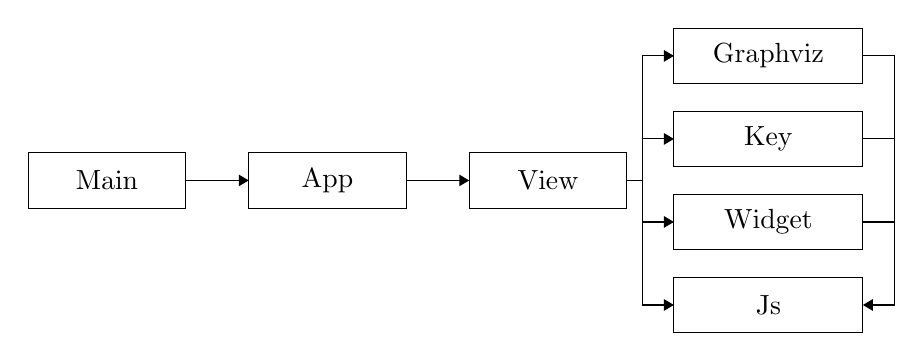
\begin{tikzpicture}
  [start chain=1 going below]

  \node (Main) [draw,header=2cm,outer ysep=50pt]               {Main};
  \node (App)  [draw,header=2cm,outer ysep=50pt,rightof2=Main] {App};
  \node (View) [draw,header=2cm,outer ysep=50pt,rightof2=App]  {View};

  \draw [->] (Main) -- (App);
  \draw [->] (App) -- (View);

  \node (Graphviz) [draw,on chain=1,field=2cm,outer ysep=5pt,rightof2=View] {Graphviz};
  \node (Key)      [draw,on chain=1,field=2cm,outer ysep=5pt]               {Key};
  \node (Widget)   [draw,on chain=1,field=2cm,outer ysep=5pt]               {Widget};
  \node (Js)       [draw,on chain=1,field=2cm,outer ysep=5pt]               {Js};

  \draw (View.east) -- ([xshift=-4mm] Js.west|-View);
  \draw [->] ([xshift=-4mm] Js.west|-View) |- (Graphviz.west);
  \draw [->] ([xshift=-4mm] Js.west|-View) |- (Js.west);
  \draw [->] ([xshift=-4mm] Js.west|-View) |- (Key.west);
  \draw [->] ([xshift=-4mm] Js.west|-View) |- (Widget.west);

  \draw [->] (Graphviz.east) -| ([xshift=4mm] Graphviz.east|-Js.east) -- (Js.east);
  \draw (Key.east)    -| ([xshift=4mm] Key.east|-Js.east);
  \draw (Widget.east) -| ([xshift=4mm] Widget.east|-Js.east);
\end{tikzpicture}

% ==============================================================================

\section{Core}
\label{sec:core-architecture}

\paragraph{The Environment} ~

\begin{tikzpicture*}{\textwidth}
  [start chain=1 going below
  ,start chain=2 going below
  ,start chain=3 going below
  ,start chain=4 going below
  ,start chain=5 going below]

  \node (Model_t) [header] {\large Model.t};

  \node (Editor_t)             [on chain=1,header,rightof=Model_t] {\large Editor.t};
  \node (Editor_id)            [on chain=1,field]                  {id};
  \node (Editor_graph)         [on chain=1,field]                  {graph};
  \node (Editor_cursor)        [on chain=1,field]                  {cursor};
  \node (Editor_actions)       [on chain=1,field]                  {actions};
  \node (Editor_known_actions) [on chain=1,field]                  {known\_actions};
  \node (Editor) [draw,fit=(Editor_id) (Editor_known_actions)] {};

  \draw [->] ([xshift=-2mm] Model_t.east) -- (Editor_t.west);

  \node (EA)                [on chain=2,header,rightof=Editor_t] {};
  \node (EA_Uuid_Id_t)      [on chain=2,field]  {Uuid.Id.t};
  \node (EA_Graph_t)        [on chain=2,field]  {Graph.t};
  \node (EA_Cursor_t)       [on chain=2,field]  {Cursor.t};
  \node (EA_Graph_action_t) [on chain=2,field2] {Graph\_action.t};

  \draw [->] (Model_t.north) |- ([yshift=3mm] Editor_t.north) -| (EA_Uuid_Id_t.north);

  \draw [->] ([xshift=-2mm] Editor_id.east)     -- ([xshift=2mm] EA_Uuid_Id_t.west);
  \draw [->] ([xshift=-2mm] Editor_graph.east)  -- ([xshift=2mm] EA_Graph_t.west);
  \draw [->] ([xshift=-2mm] Editor_cursor.east) -- ([xshift=2mm] EA_Cursor_t.west);
  \draw ([xshift=-2mm] Editor_actions.east)       -| ([xshift=-2mm] EA_Graph_action_t.west);
  \draw ([xshift=-2mm] Editor_known_actions.east) -| ([xshift=-2mm] EA_Graph_action_t.west);
  \draw [->] ([xshift=-2mm] EA_Graph_action_t.west) -- ([xshift=2mm] EA_Graph_action_t.west);

  \node (Action_t)         [on chain=3,header,rightof=EA] {\large Action.t};
  \node (Action_editor_id) [on chain=3,field]             {editor\_id};
  \node (Action_action)    [on chain=3,field]             {action};
  \node [draw,fit=(Action_editor_id) (Action_action)] {};

  \draw [->] ([xshift=2mm] Action_editor_id.west) -- ([xshift=-2mm] EA_Uuid_Id_t.east);

  \node (Action_t')   [on chain=4,header,rightof=Action_t] {};
  \node (Action_edit) [on chain=4,field]                   {Action.edit};
  \node (Action_comm) [on chain=4,field]                   {Action.comm};
  \node (Action_move) [on chain=4,field]                   {Action.move};

  \draw [->] ([xshift=-2mm] Action_action.east) -- ([xshift=2mm] Action_comm.west);
  \draw [->] ([xshift=2mm] Action_action.east)  |- ([xshift=2mm] Action_edit.west);
  \draw [->] ([xshift=2mm] Action_action.east)  |- ([xshift=2mm] Action_move.west);

  \draw [->] (Action_move.south) |- ([yshift=-3mm] EA_Cursor_t.south) -- (EA_Cursor_t.south);
  \draw [->] ([xshift=-2mm] Action_comm.east)
  -| ([xshift=2mm] Action_comm.east|-EA_Graph_action_t.east)
  -- ([xshift=-2mm] EA_Graph_action_t.east);

  \node (AA_Lang_Constructor_t) [on chain=5,header=4cm,rightof4=Action_t'] {Lang.Constructor.t};
  \node (AA_Vertex_t)           [on chain=5,field=4cm]                     {Vertex.t};
  \node (AA_empty)              [on chain=5,field=4cm]                     {};
  \node (State_t)               [on chain=5,field2=4cm]                    {\large State.t};

  \draw [->] ([xshift=-2mm] Action_edit.east) -- ([xshift=2mm] AA_Vertex_t.west);
  \draw [->] ([xshift=2mm] Action_edit.east) |- ([xshift=2mm] AA_Lang_Constructor_t);
\end{tikzpicture*}

\paragraph{The Graph} ~

\nopagebreak

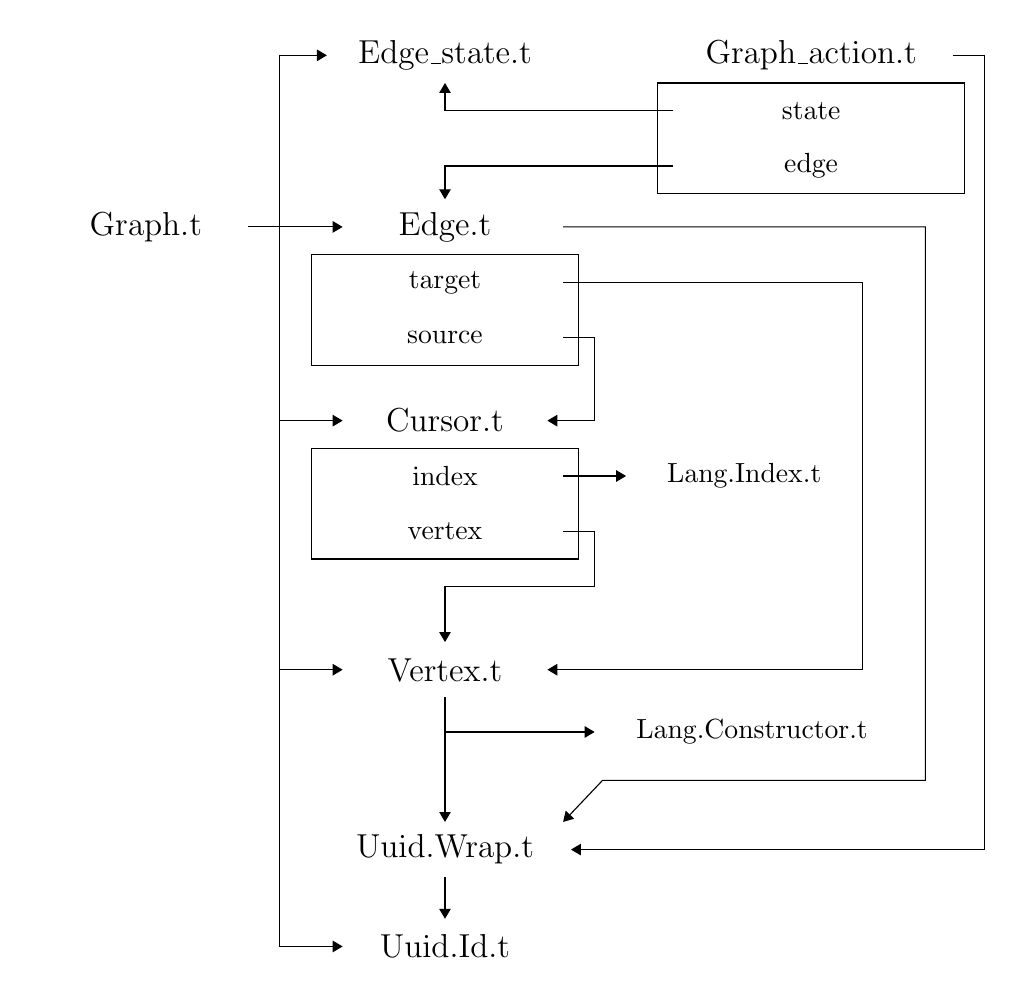
\begin{tikzpicture}
  [start chain=1 going below
  ]
  \node (Graph_t) [header] {\large Graph.t};

  \node (Edge_t) [header,right=8mm of Graph_t] {\large Edge.t};
  \node (Edge_target) [field,below=0mm of Edge_t.south]      {target};
  \node (Edge_source) [field,below=0mm of Edge_target.south] {source};
  \node (Edge) [draw,fit=(Edge_target) (Edge_source)] {};

  \node (Edge_state_t) [header,above=42pt of Edge_t] {\large Edge\_state.t};

  \node (Cursor_t) [header,below=10pt of Edge,anchor=north] {\large Cursor.t};
  \node (Cursor_index) [field,below=0mm of Cursor_t,anchor=north] {index};
  \node (Cursor_vertex) [field,below=0mm of Cursor_index,anchor=north] {vertex};
  \node (Cursor) [draw,fit=(Cursor_index) (Cursor_vertex)] {};

  \draw [->] ([xshift=-2mm] Edge_source.east) -- ([xshift=2mm] Edge_source.east)
  |- ([xshift=-2mm] Cursor_t.east);

  \node (Lang_Index_t) [field,right=4mm of Cursor_index.east] {Lang.Index.t};
  \draw [->] ([xshift=-2mm] Cursor_index.east) -- ([xshift=2mm] Lang_Index_t.west);

  \node (Vertex_t) [header,below=30pt of Cursor.south,anchor=north] {\large Vertex.t};
  \draw [->] ([xshift=-2mm] Cursor_vertex.east)
  -- ([xshift=2mm] Cursor_vertex.east)
  -- ([xshift=2mm,yshift=-20pt] Cursor_vertex.east)
  -| (Vertex_t.north);
  \draw [->] ([xshift=-2mm] Edge_target.east)
  -- ([xshift=3.6cm] Edge_target.east)
  |- ([xshift=-2mm] Vertex_t.east);

  \node (Uuid_Wrap_t) [header,below=45pt of Vertex_t.south,anchor=north] {\large Uuid.Wrap.t};
  \draw [->] (Vertex_t.south) -- (Uuid_Wrap_t.north);
  \draw [->] (Edge_t.east)
  -- ([xshift=4.6cm] Edge_t.east)
  -- ([xshift=4.6cm,yshift=-30pt] Edge_t.east|-Vertex_t.south)
  -- ([xshift=5mm,yshift=-30pt] Edge_t.east|-Vertex_t.south)
  -- (Uuid_Wrap_t.north east);

  \node (Uuid_Id_t) [header,below=15pt of Uuid_Wrap_t.south,anchor=north] {\large Uuid.Id.t};
  \draw [->] (Uuid_Wrap_t.south) -- (Uuid_Id_t.north);

  \node (Lang_Constructor_t) [header=4cm,below right=12.5pt and 4mm of Vertex_t.east] {Lang.Constructor.t};
  \draw [->] (Vertex_t.south|-Lang_Constructor_t.west) -- (Lang_Constructor_t.west);

  \draw [->] ([xshift=-2mm] Graph_t.east) -- ([xshift=2mm] Edge_t.west);
  \draw [->] ([xshift=2mm] Graph_t.east) |- (Edge_state_t.west);
  \draw [->] ([xshift=2mm] Graph_t.east) |- ([xshift=2mm] Cursor_t.west);
  \draw [->] ([xshift=2mm] Graph_t.east) |- ([xshift=2mm] Vertex_t.west);
  \draw [->] ([xshift=2mm] Graph_t.east) |- ([xshift=2mm] Uuid_Id_t.west);

  \node (Graph_action_t) [header=4cm,right=1.15cm of Edge_state_t.east] {\large Graph\_action.t};
  \node (Graph_action_state) [field=3.5cm,below=0mm of Graph_action_t.south] {state};
  \node (Graph_action_edge) [field=3.5cm,below=0mm of Graph_action_state.south] {edge};
  \node (Graph_action) [draw,fit=(Graph_action_state) (Graph_action_edge)] {};

  \draw [->] ([xshift=2mm] Graph_action_edge.west) -| (Edge_t.north);

  \draw [->] ([xshift=2mm] Graph_action_state.west)
  -| (Edge_state_t.south);

  \draw [->] ([xshift=-2mm] Graph_action_t.east)
  -- ([xshift=2mm] Graph_action_t.east)
  |- ([xshift=1mm] Uuid_Wrap_t.east);
\end{tikzpicture}

% ##############################################################################

\chapter{Implementation}
\label{chap:implementation}

% ==============================================================================

\section{Sets and Relations}
\label{sec:sets-and-relations-implementation}

Hello, this is a test


\section{Editor}
\label{sec:editor-implementation}


Talk about how the editor is implemented




\end{document}
